\documentclass[aspectratio=169,10pt]{beamer}
\usepackage{graphicx}
\usepackage{booktabs}
\usepackage{amsmath}
\graphicspath{{figures/}}

%,- red colour theme,-
\definecolor{ubred}{RGB}{160,20,20}
\definecolor{ubdark}{RGB}{90,10,10}
\definecolor{ublight}{RGB}{205,70,70}
\usetheme{default}
\usecolortheme{default}
\setbeamercolor{structure}{fg=ubred}
\setbeamercolor{title}{fg=ubdark}
\setbeamercolor{frametitle}{fg=white,bg=ubred}
\setbeamercolor{section in head/foot}{fg=white,bg=ubdark}
\setbeamercolor{alerted text}{fg=ubred}
\setbeamercolor{block title}{fg=white,bg=ubred}
\setbeamercolor{block body}{bg=ubred!8}
\setbeamercolor{itemize item}{fg=ubred}
\setbeamercolor{itemize subitem}{fg=ublight}
\setbeamertemplate{navigation symbols}{}
\setbeamertemplate{frametitle}{\vskip4pt\usebeamercolor[fg]{frametitle}%
  \begin{beamercolorbox}[wd=\paperwidth,ht=2.4ex,dp=1ex,leftskip=.3cm]{frametitle}%
  \bfseries\insertframetitle\end{beamercolorbox}}
%,- footline with page number,-
\setbeamertemplate{footline}{%
  \leavevmode\hbox{%
  \begin{beamercolorbox}[wd=.62\paperwidth,ht=2.4ex,dp=1ex,leftskip=.3cm]{section in head/foot}%
  \usebeamerfont{author in head/foot}\insertshortauthor\ | MicroBooNE NuMI CC$1\mu1\pi^{\pm}$\hfill\end{beamercolorbox}%
  \begin{beamercolorbox}[wd=.38\paperwidth,ht=2.4ex,dp=1ex,rightskip=.3cm]{section in head/foot}%
  \hfill\insertshorttitle\quad\insertframenumber\,/\,\inserttotalframenumber\end{beamercolorbox}}}

\title[CC$1\mu1\pi^{\pm}$]{Differential CC$\,1\mu1\pi^{\pm}$ cross sections on argon in the NuMI beam}
\subtitle{Status of the blind analysis and a request to open the control regions}
\author[Pophale, Nowak]{Ishanee Pophale and Jarek Nowak}
\institute{Lancaster University}
\date{MicroBooNE Collaboration Meeting, Imperial College London, 12--17 September 2026}
\newcommand{\uboone}{MicroBooNE}
\newcommand{\GeVc}{~GeV/$c$}

\begin{document}

{\setbeamertemplate{footline}{}
\begin{frame}[plain]
  \titlepage
  \begin{center}\small\color{ubdark}
  $\nu_\mu+\bar\nu_\mu$ CC single charged pion on argon \;$\bullet$\; FHC, RHC and combined \;$\bullet$\; blind, fake-data results
  \end{center}
\end{frame}}

% ---------------------------------------------------------------------------
\begin{frame}{What is measured}
  \begin{columns}[T]
  \column{.56\textwidth}
  \small\textbf{Signal} (truth level, charge-blind): $\nu_\mu/\bar\nu_\mu$ CC in the FV with exactly one $\mu$,
  exactly one $\pi^\pm$, no $\pi^0$, no kaons or other mesons, any number of nucleons; coherent production included.\\[2pt]
  \textbf{Measured phase space}: $p_\mu>0.15$, $p_\pi>0.175$\GeVc, $\theta_{\mu\pi}<2.6$~rad
  \vspace{2pt}
  \begin{block}{Deliverables per configuration (FHC, RHC, combined)}
    \footnotesize
    \begin{itemize}\itemsep1pt
      \item total flux-averaged cross section (cut-and-count)
      \item $d\sigma/dp_\mu$, $d\sigma/d\cos\theta_\mu$ and $d\sigma/d\theta_\mu$,
            $d\sigma/d\cos\theta_\pi$, $d\sigma/d\theta_{\mu\pi}$, two-bin $d\sigma/dp_\pi$
      \item proton-tagged subsample: integrated cross section (headline); TKI and $W_{\rm had}$ as secondary results
    \end{itemize}
  \end{block}
  \column{.42\textwidth}
  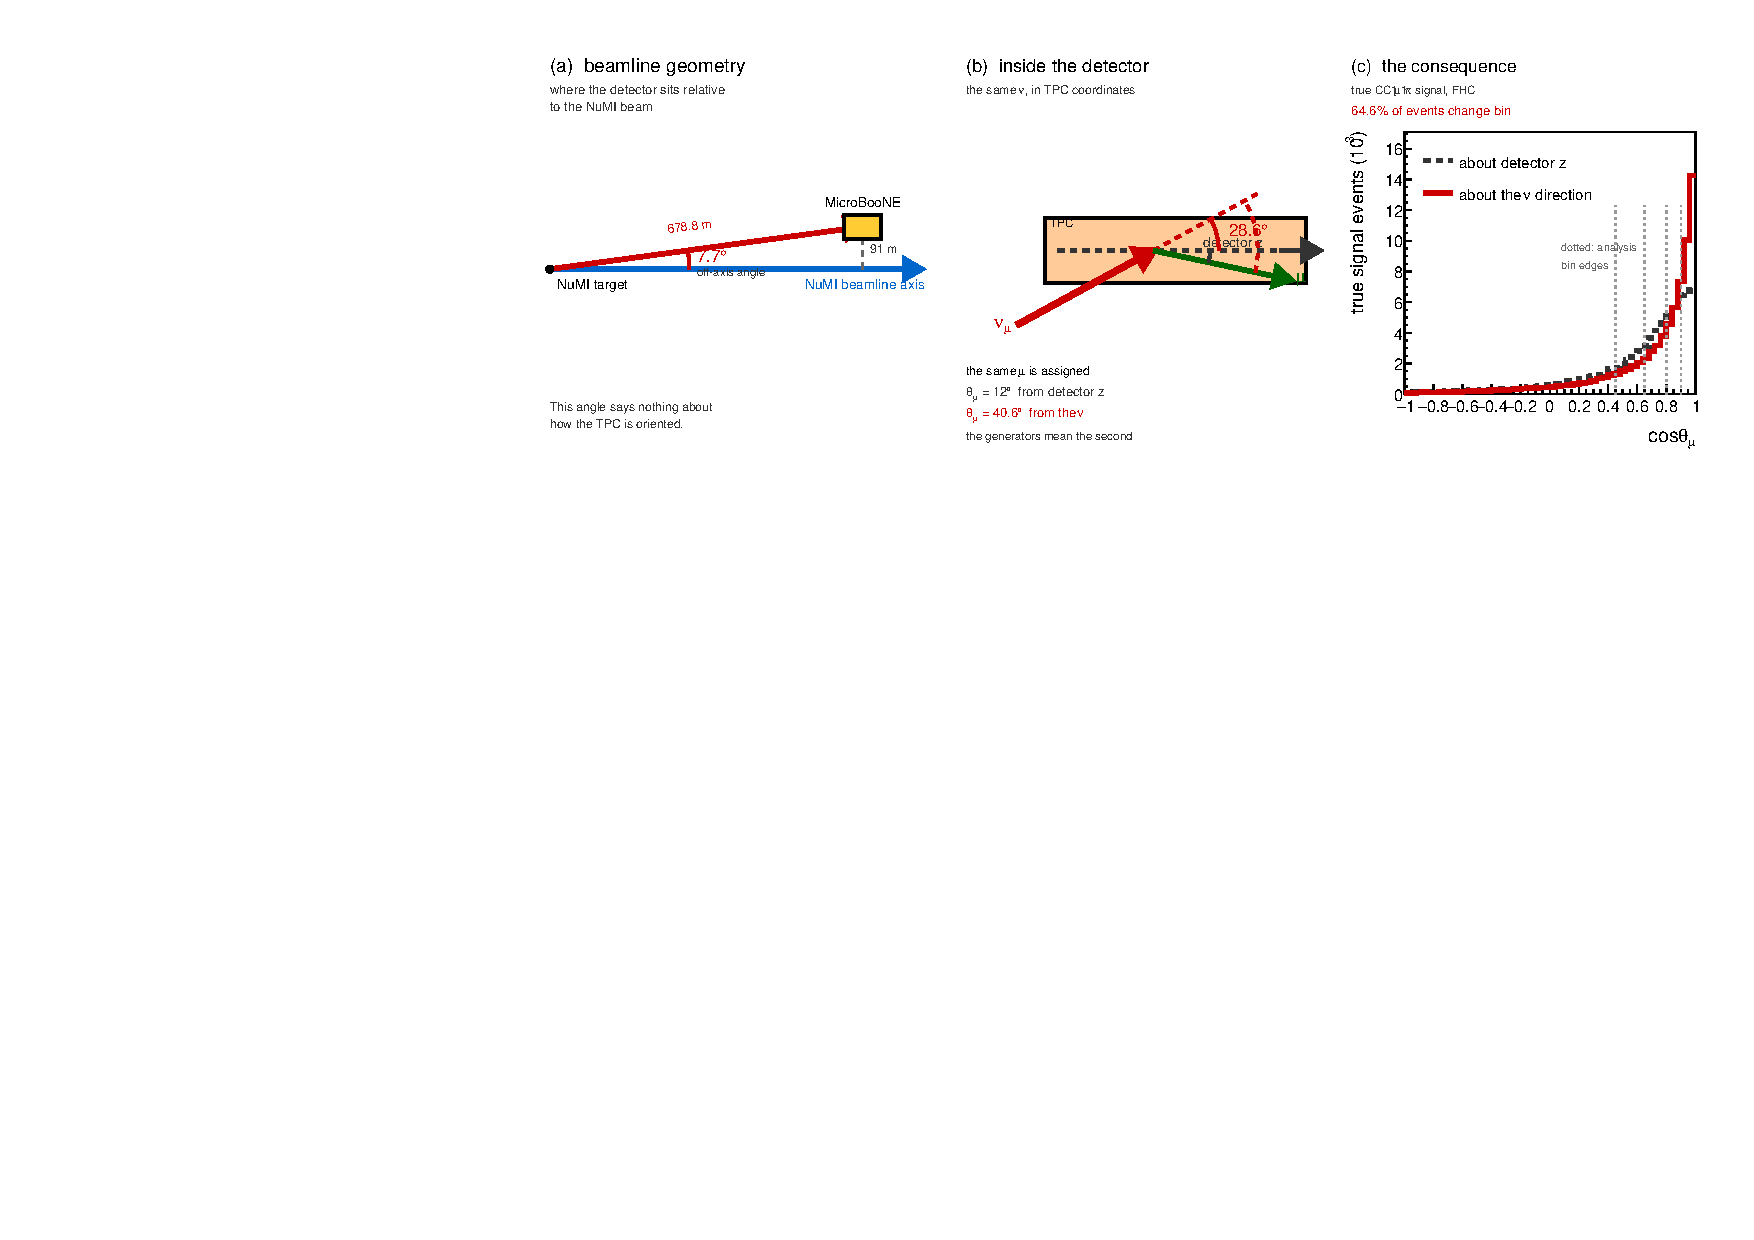
\includegraphics[width=\textwidth]{numi_geometry}\\
  {\footnotesize \uboone{} sits $7.7^\circ$ off the NuMI axis; the beam arrives $28^\circ$ from detector $z$, so all angles and transverse quantities are computed in the beam frame.}
  \end{columns}
  \vspace{3pt}
  \alert{Blind analysis}: every ``data'' point in this talk is Poisson-thrown central-value MC. No beam-on signal region has been opened.
\end{frame}

% ---------------------------------------------------------------------------
\begin{frame}{Exposure, normalisation and beam-off}
  \begin{columns}[T]
  \column{.5\textwidth}
  \small
  \begin{tabular}{lcc}
  \toprule
  Configuration & Runs & Data POT ($10^{20}$) \\
  \midrule
  FHC & 1, 2, 4, 5 & 8.857 \\
  RHC & 1, 2, 3, 4a--c & 11.082 \\
  Combined & all 14 overlay files & 19.939 \\
  \bottomrule
  \end{tabular}
  \vspace{4pt}
  \begin{itemize}\itemsep2pt
    \item every run scaled by its own data/MC POT; combined = per-mode data exposures
    \item per-configuration integrated flux (new-G4, $E_\nu>60$~MeV): FHC $6.81$, RHC $6.45$, comb.\ $6.61\times10^{-10}$~cm$^{-2}$/POT
    \item $N_{\rm Ar}=8.71\times10^{29}$ (dead $z$ slab removed)
    \item CV weight = tune $\times$ PPFX $\times$ normalisation, one safe-weight rule everywhere
  \end{itemize}
  \column{.5\textwidth}
  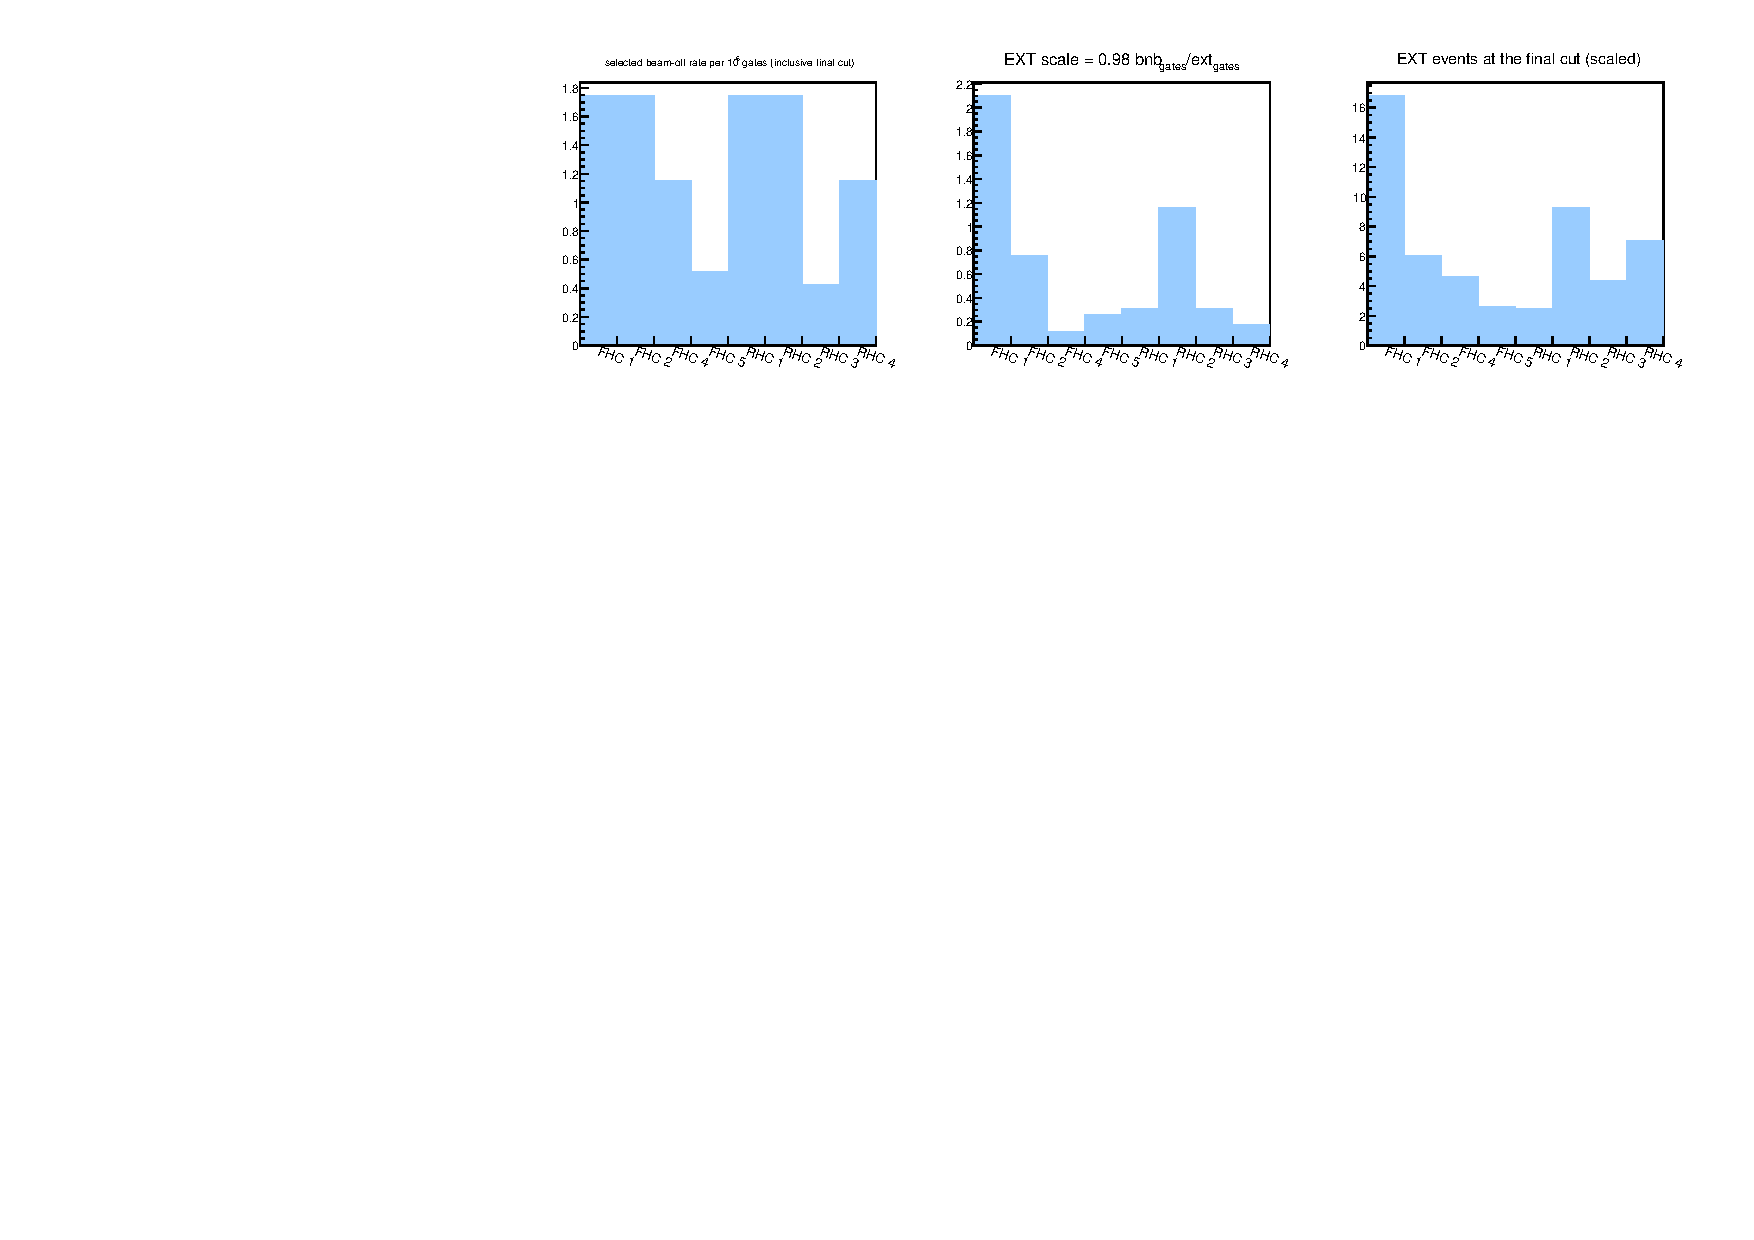
\includegraphics[width=\textwidth]{ext_perrun_validation}\\
  {\footnotesize \textbf{Beam-off}: cosmic-only, matched by run period (horn label irrelevant), each run scaled by its beam-on/beam-off \emph{gate} ratio. The pre-CRT Run-1 rate is $3$--$4\times$ the CRT-era one. EXT is $1.9\%$ of the final sample (30 FHC events).}
  \end{columns}
\end{frame}

% ---------------------------------------------------------------------------
\begin{frame}{Selection and yields}
  \begin{columns}[T]
  \column{.5\textwidth}
  \small
  \textbf{Cuts}: software trigger, vertex in FV, topological score $>0.67$, muon candidate (highest muon-BDT score among qualifying tracks),
  exactly one contained pion candidate (LLR, MIP-BDT, pion-BDT, Bragg-$\pi$), three-plane hits, shower veto,
  $\theta_{\mu\pi}<2.6$~rad, non-proton multiplicity $<4$ and $<5$ tracks.
  \vspace{4pt}
  \begin{tabular}{lrrrrr}
  \toprule
  Final cut & Signal & $\nu$ bkg & EXT & Pred. & Pur. \\
  \midrule
  FHC & 943 & 637 & 30 & 1\,612 & 58.5\% \\
  RHC & 1\,015 & 720 & 23 & 1\,759 & 57.7\% \\
  Comb. & 1\,959 & 1\,357 & 53 & 3\,372 & 58.1\% \\
  \bottomrule
  \end{tabular}\\[2pt]
  Efficiency $17.4$--$17.6\%$ in the measured phase space; largest background: CC$0\pi$ with a proton taken as the pion.
  \column{.5\textwidth}
  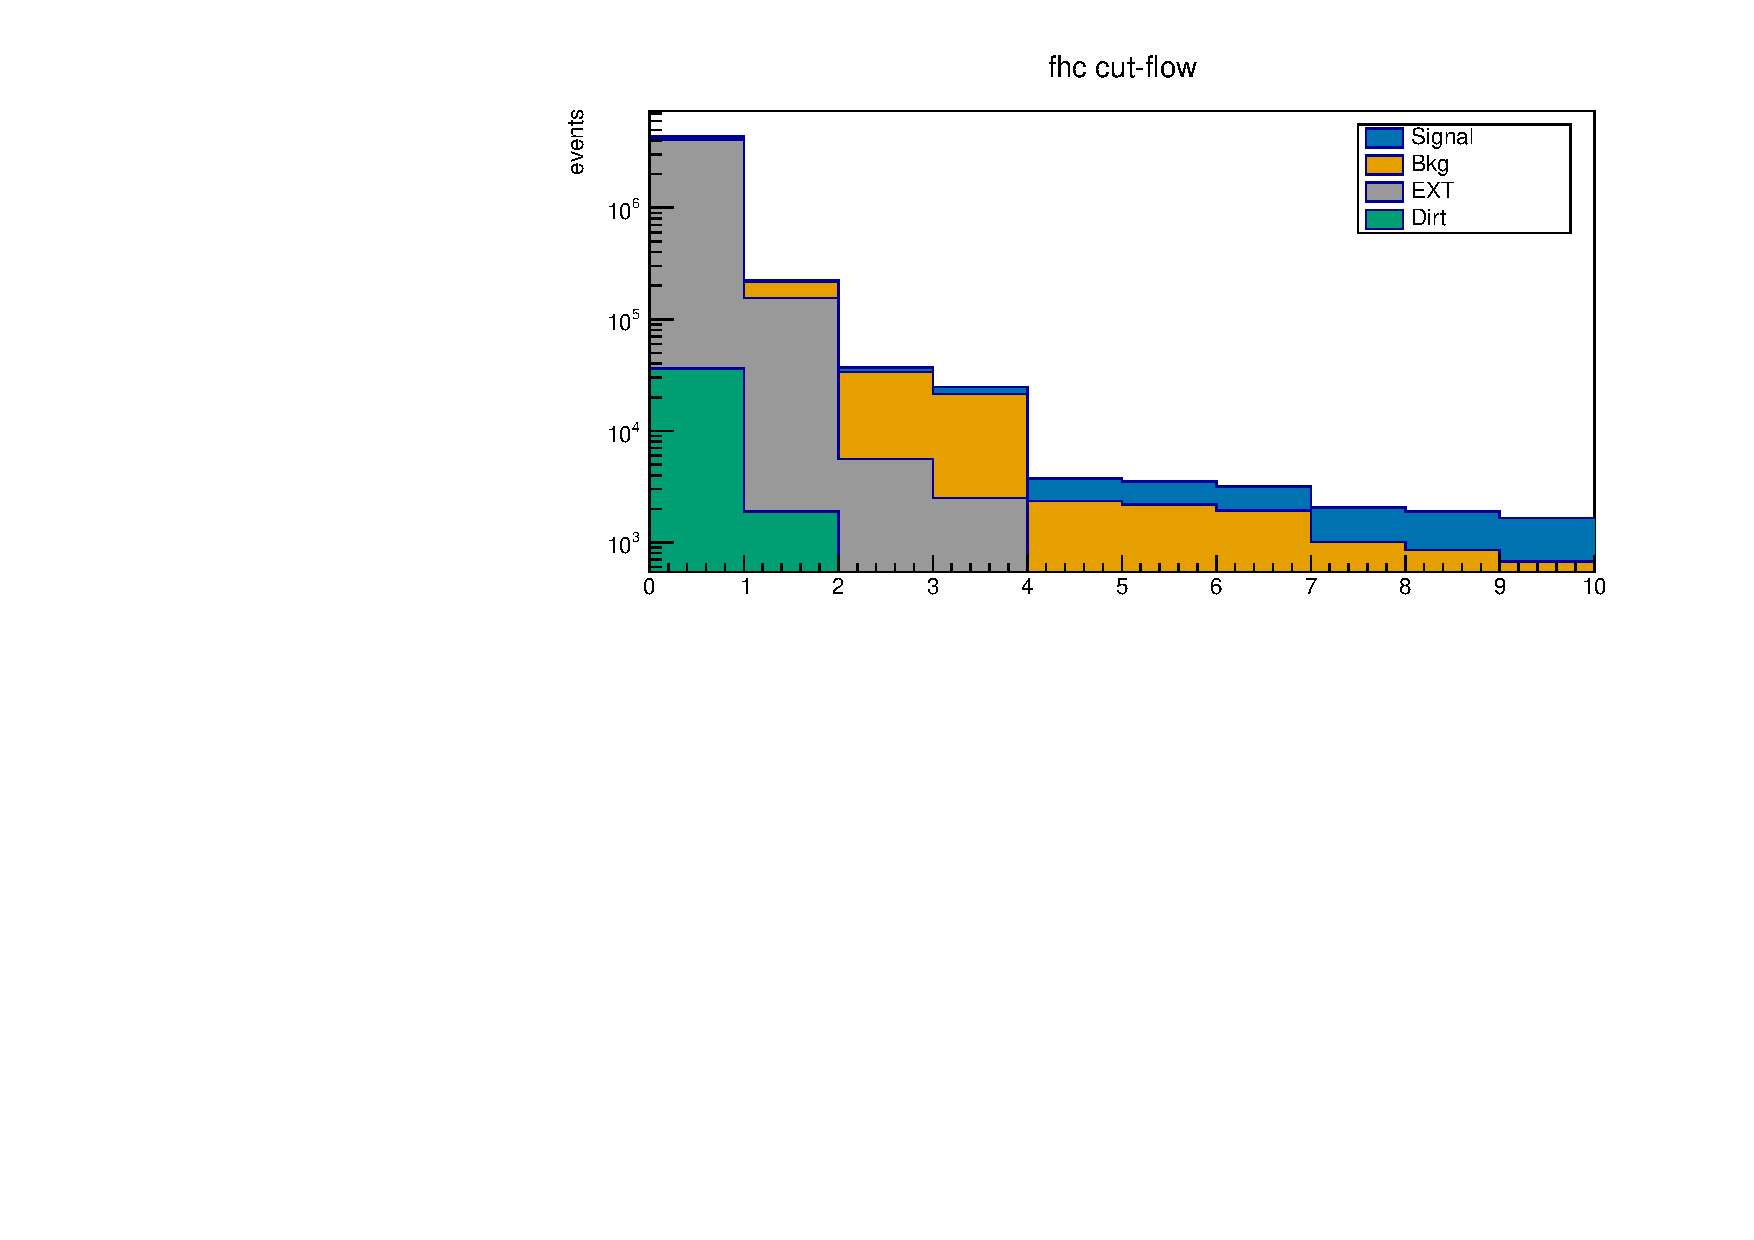
\includegraphics[width=\textwidth]{cutflow_yields_fhc}\\
  {\footnotesize FHC cut-flow, per-run POT-scaled, full CV weight.}
  \end{columns}
\end{frame}

% ---------------------------------------------------------------------------
\begin{frame}{The pion momentum sets the scope}
  \begin{columns}[T]
  \column{.48\textwidth}
  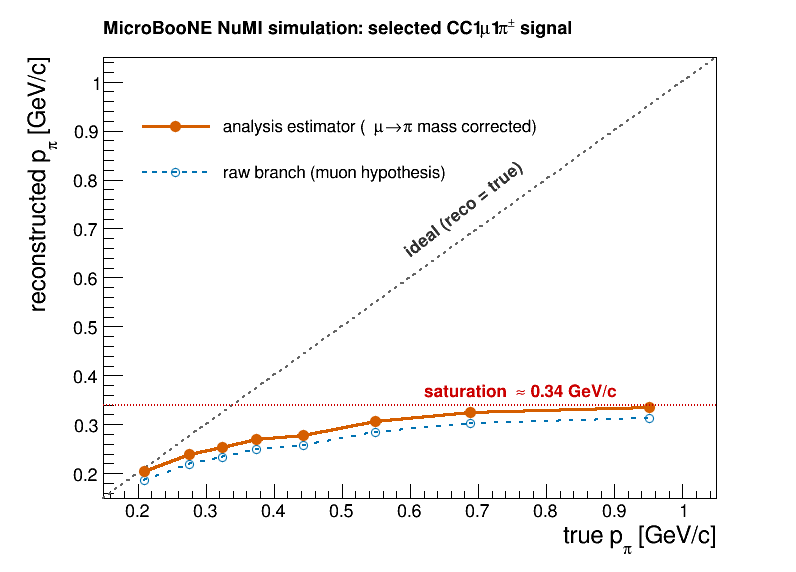
\includegraphics[width=\textwidth]{ppi_saturation}\\
  {\footnotesize Reconstructed $p_\pi$ (range under the muon hypothesis, mass-corrected) saturates near $0.34$\GeVc: pions interact before stopping.}
  \column{.52\textwidth}
  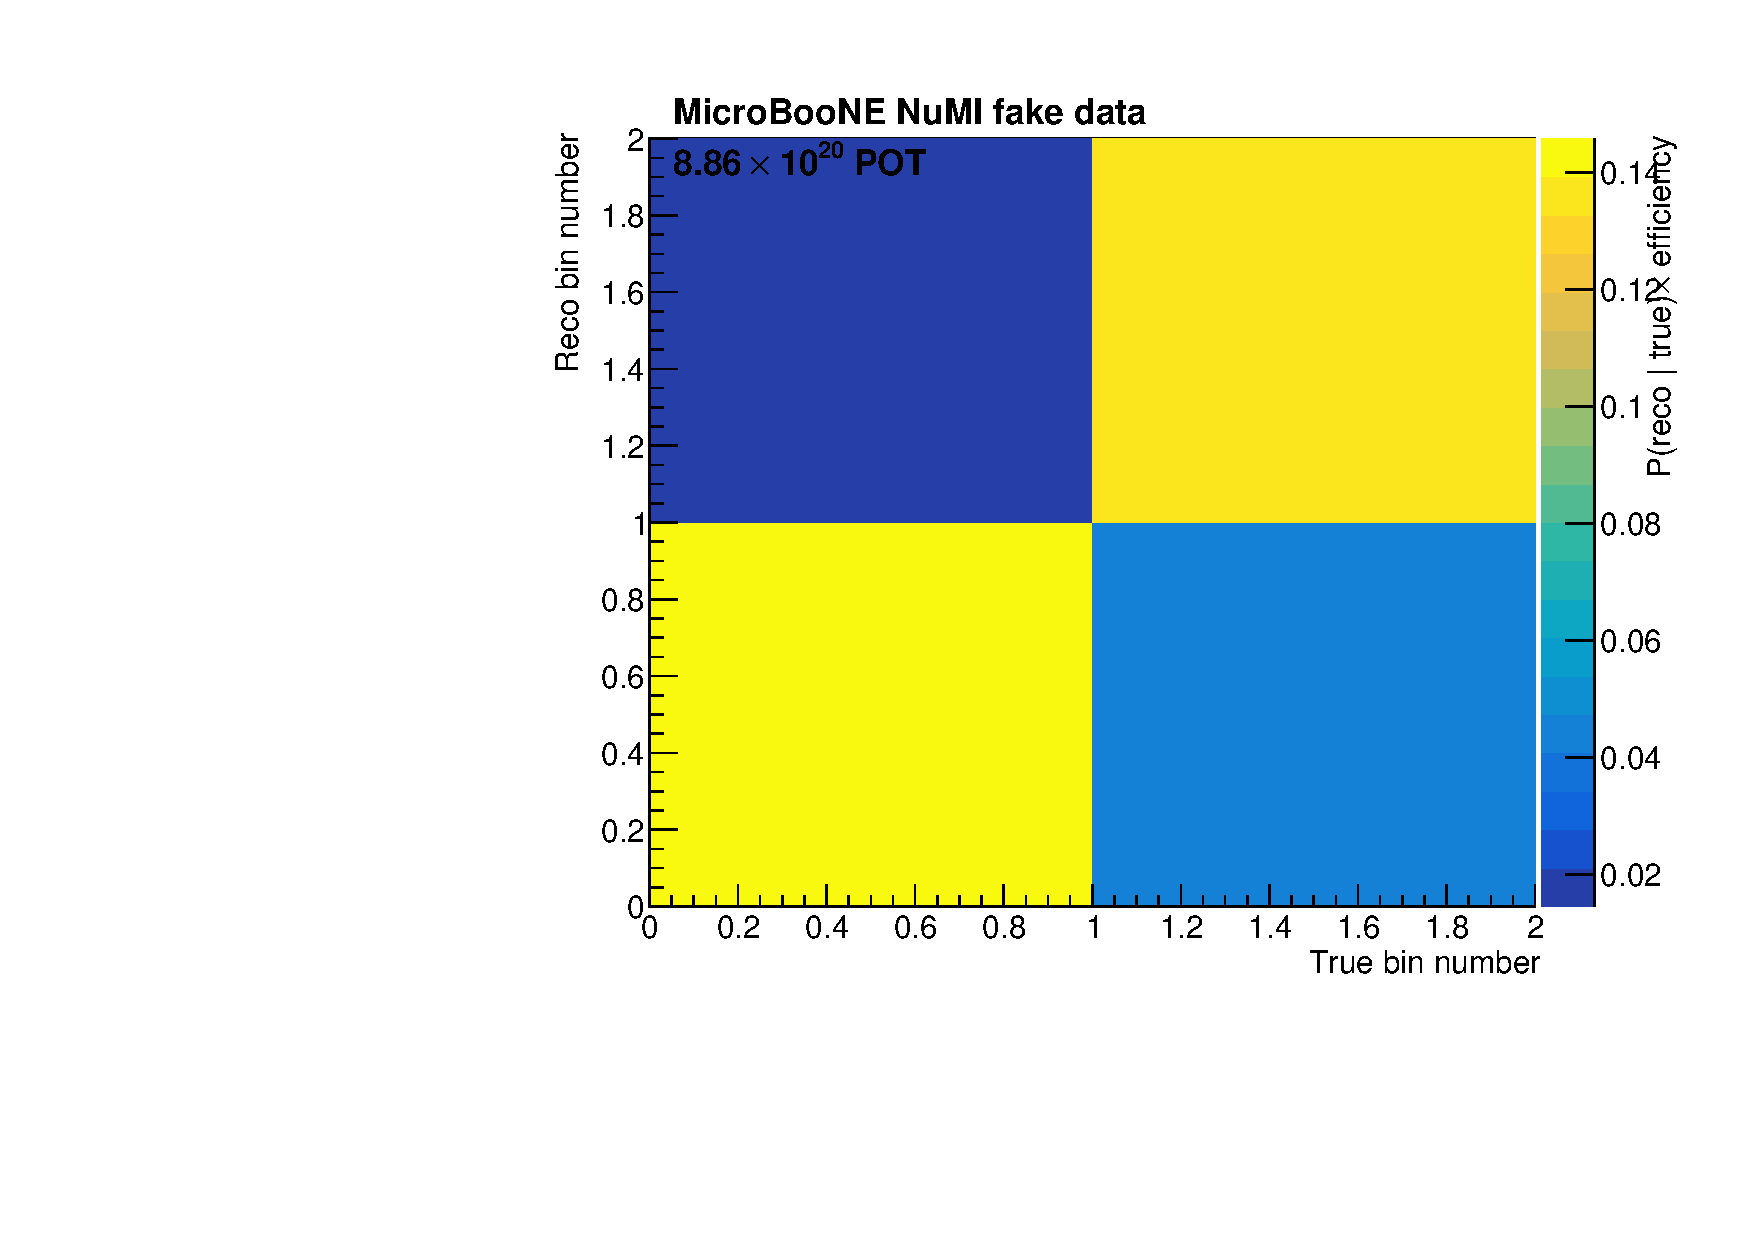
\includegraphics[width=.49\textwidth]{fw_resp_ppi}\hfill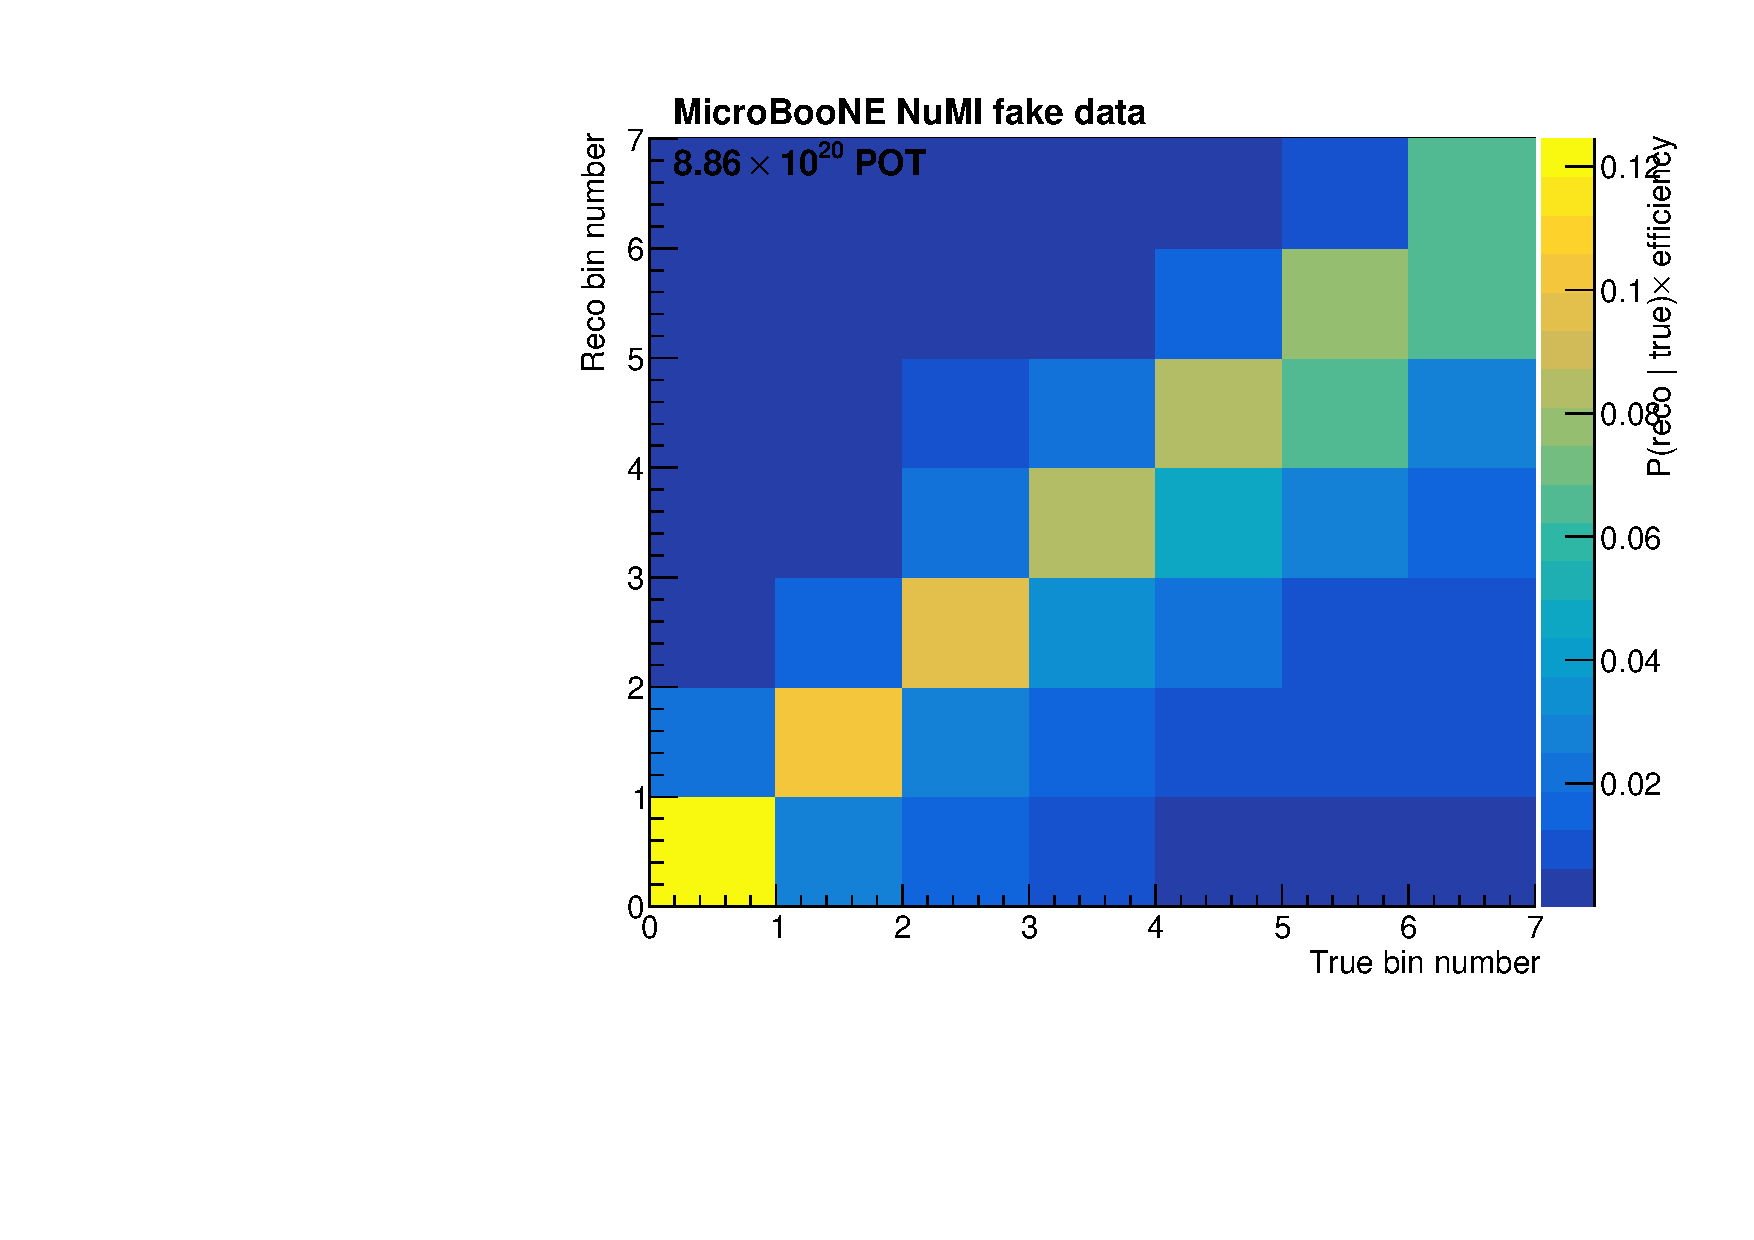
\includegraphics[width=.49\textwidth]{fw_resp_pmu}\\
  {\footnotesize Smearceptance $S=\varepsilon M$: five-bin $p_\pi$ (diagnostic, left) vs.\ $p_\mu$ (right).}
  \vspace{4pt}\small
  \begin{itemize}\itemsep2pt
    \item every estimator tried (golden-pion tag, MCS, calorimetry, regression, daughter recovery): a physics limit, not an algorithmic one
    \item $p_\pi$ released as \textbf{two bins}: $[0.175,0.205]$ and $>0.205$\GeVc, migration diagonals $91\%$ / $76\%$
    \item proton-tagged $W_{\pi p}$ shape \textbf{withdrawn}; the sample supports an integrated cross section
  \end{itemize}
  \end{columns}
\end{frame}

% ---------------------------------------------------------------------------
\begin{frame}{Extraction: Wiener-SVD and what its integral means}
  \small
  \begin{columns}[T]
  \column{.55\textwidth}
  \begin{itemize}\itemsep3pt
    \item $n^{\rm reco}=S\,N^{\rm true}+b$ with $S=\varepsilon M$ inverted once (no extra $1/\varepsilon$)
    \item Wiener-SVD (\textsc{XSecAnalyzer}), second-derivative regularisation aware of the non-uniform bin widths
    \item the result is $A_C\,x_{\rm true}$; every prediction is smeared by the released $A_C$ before comparison
    \item $A_C$ is \emph{not} norm preserving: the integral of a differential result is observable-dependent
      ($0.57$--$0.86\times10^{-38}$~cm$^2$/Ar); D'Agostini gives a flat, $\sim\!30\%$ higher integral
    \item \alert{the physical total is the cut-and-count value}
  \end{itemize}
  \column{.45\textwidth}
  \begin{block}{Total flux-averaged cross section ($10^{-38}$~cm$^2$/Ar)}
  \begin{tabular}{lcc}
  \toprule
  & inclusive & proton-tagged \\
  \midrule
  FHC  & $1.03\pm0.43$ & $0.63\pm0.31$ \\
  RHC  & $0.93\pm0.42$ & $0.55\pm0.21$ \\
  Comb.& $0.98\pm0.40$ & $0.59\pm0.25$ \\
  \bottomrule
  \end{tabular}\\[3pt]
  {\footnotesize On fake data this \emph{is} the injected tune (closure $=1$ by construction); the uncertainty is what real data will carry. RHC/FHC $=0.90$. GENIE~v3 $0.5$--$0.6\sigma$ below, GiBUU/NEUT/NuWro within $0.7\sigma$.}
  \end{block}
  \end{columns}
\end{frame}

% ---------------------------------------------------------------------------
\begin{frame}{Differential results, FHC}
  \centering
  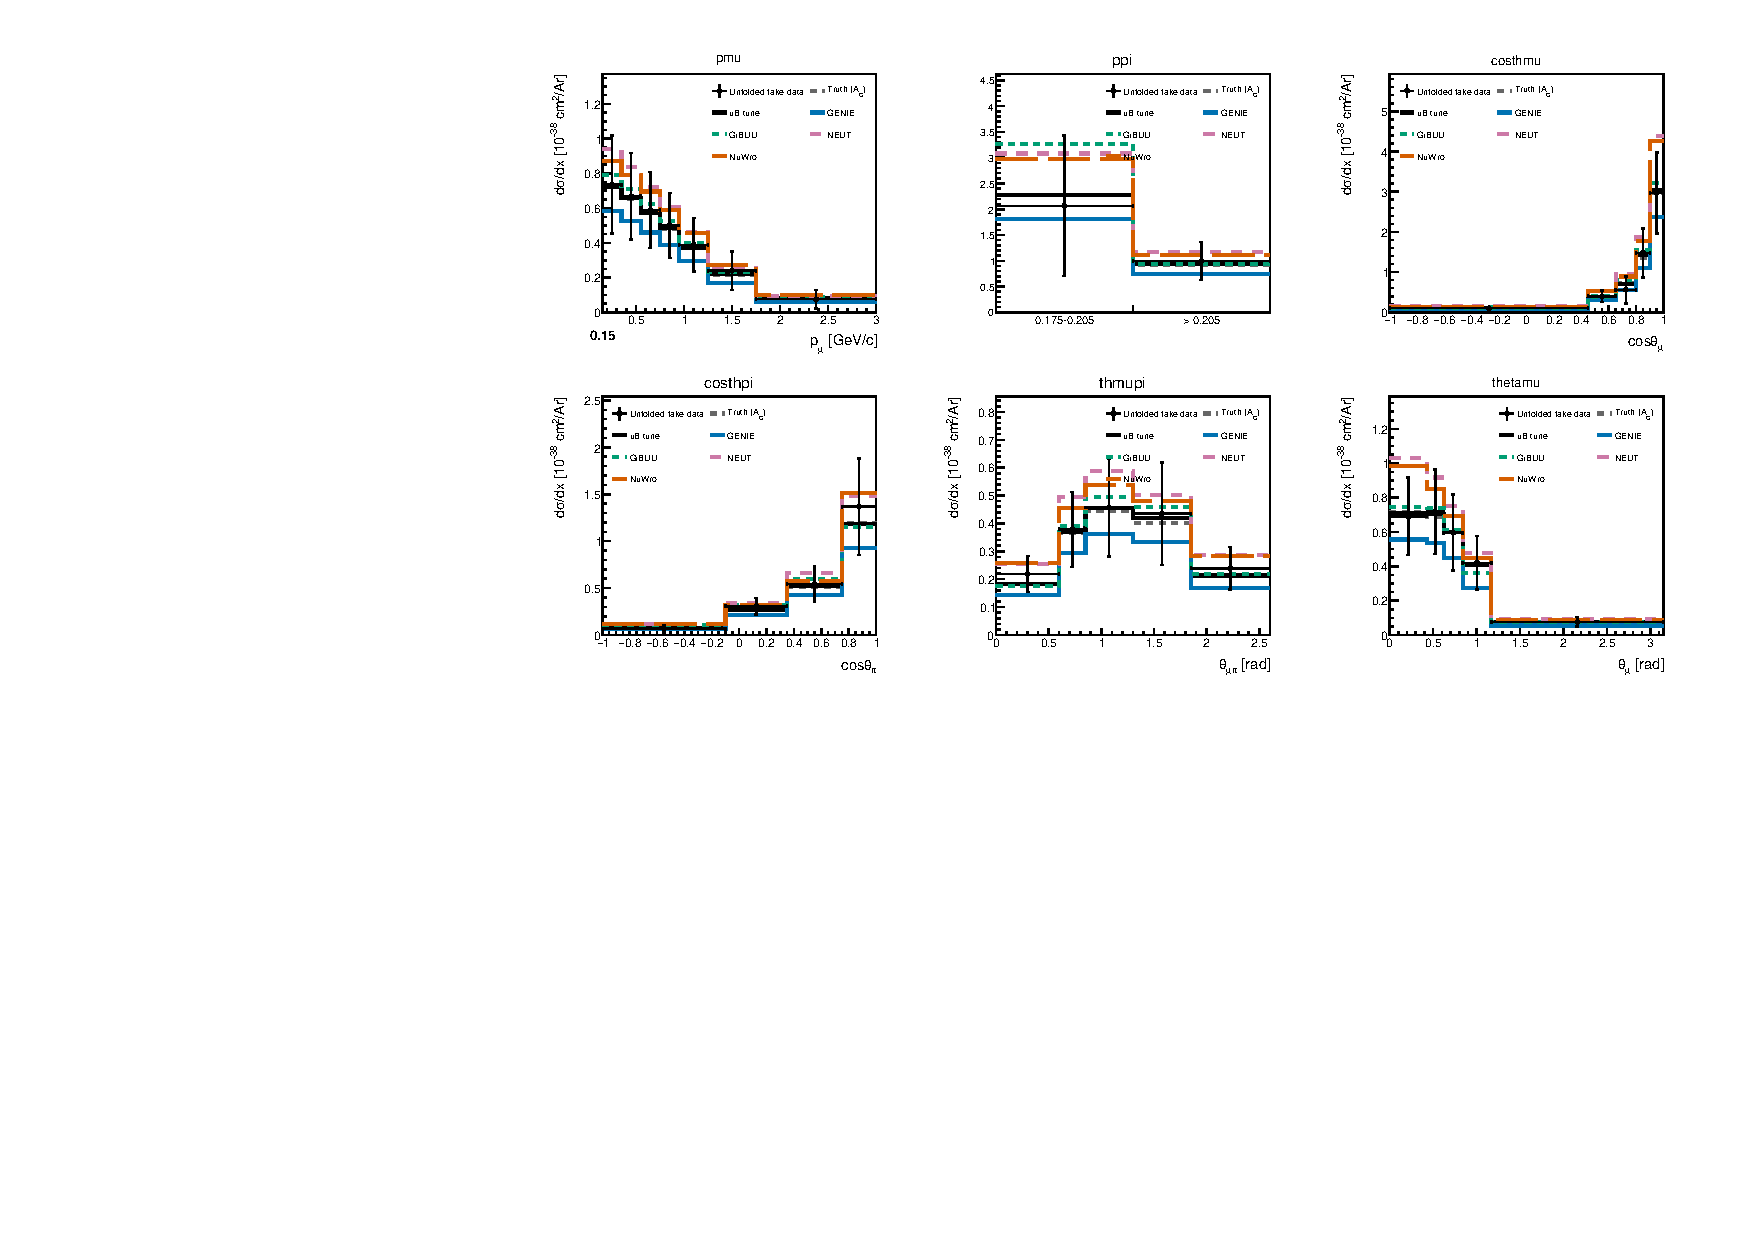
\includegraphics[width=.80\textwidth]{dsigma_FHC5}\\
  {\scriptsize Unfolded fake data, $A_C$-smeared truth, tune and the four generators, all in the $A_C$-smeared space. Generators differ by normalisation ($\times1.6$, GENIE to NEUT); shapes agree within the uncertainties. Full covariance: flux, cross section, re-interaction, detector, POT, targets, statistics.}
\end{frame}

% ---------------------------------------------------------------------------
\begin{frame}{RHC and combined}
  \begin{columns}[T]
  \column{.5\textwidth}\centering
  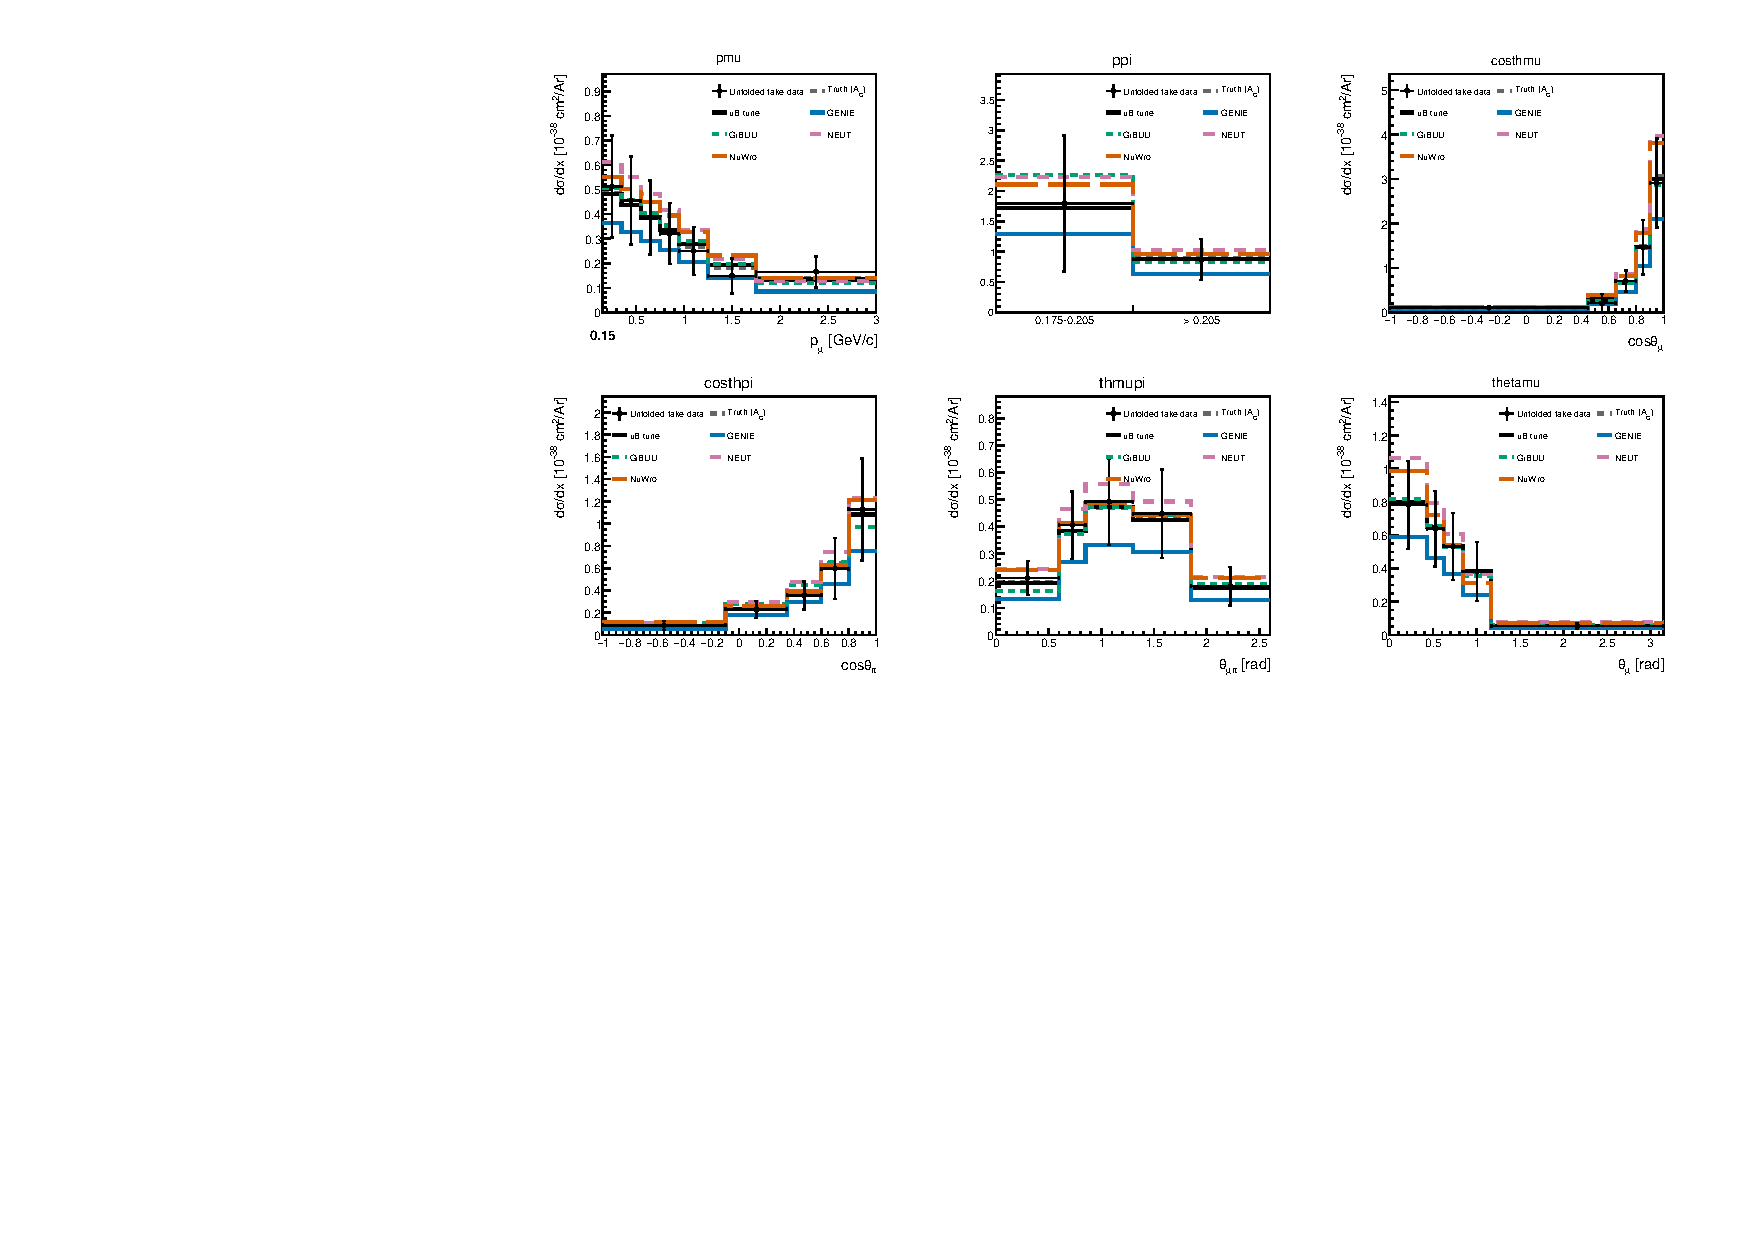
\includegraphics[width=\textwidth]{dsigma_RHCFULL}\\ {\footnotesize RHC}
  \column{.5\textwidth}\centering
  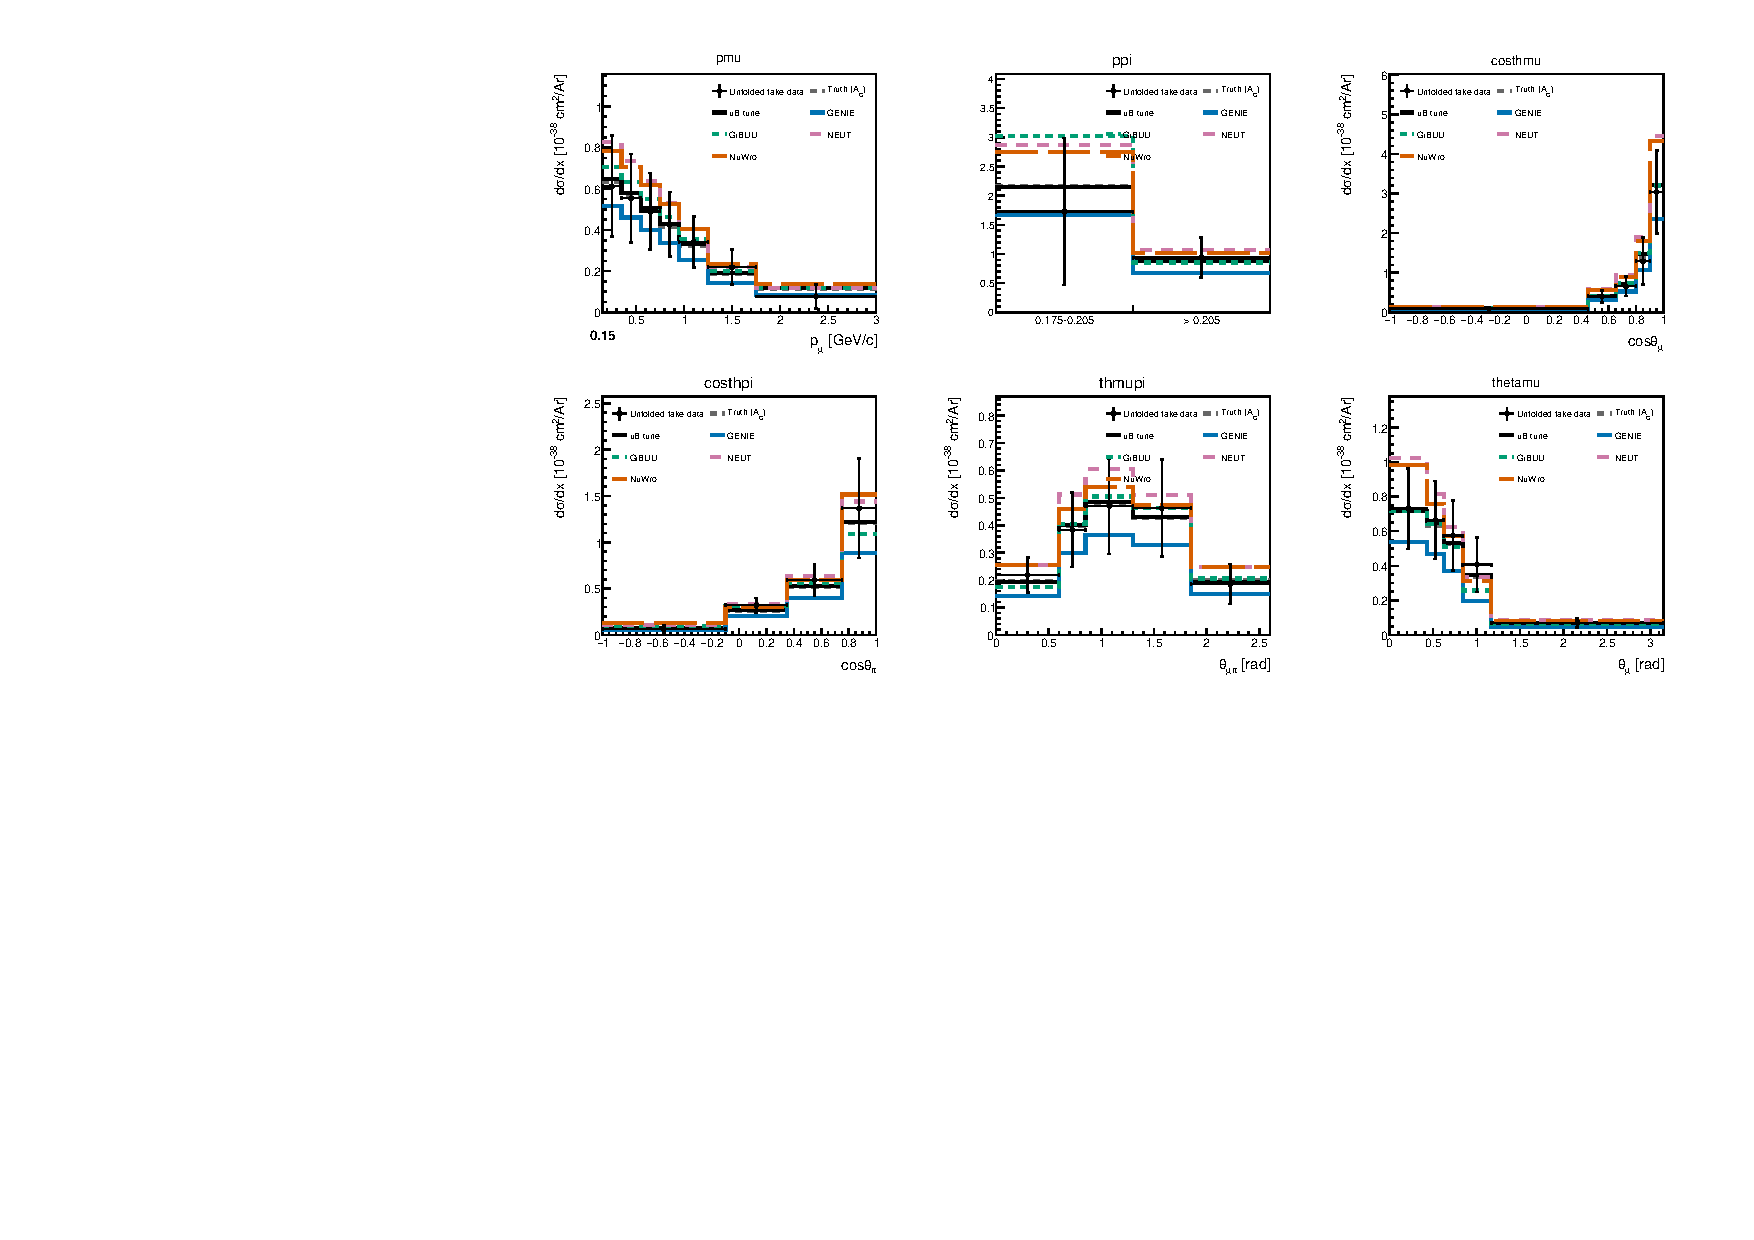
\includegraphics[width=\textwidth]{dsigma_COMB}\\ {\footnotesize Combined FHC$+$RHC}
  \end{columns}
  \vspace{3pt}\small
  Same 600 PPFX universes index-matched across both horn modes (rigorous flux correlation); native Run-4 RHC detector variations; each mode normalised to its own exposure and flux.
\end{frame}

% ---------------------------------------------------------------------------
\begin{frame}{Uncertainties}
  \begin{columns}[T]
  \column{.5\textwidth}
  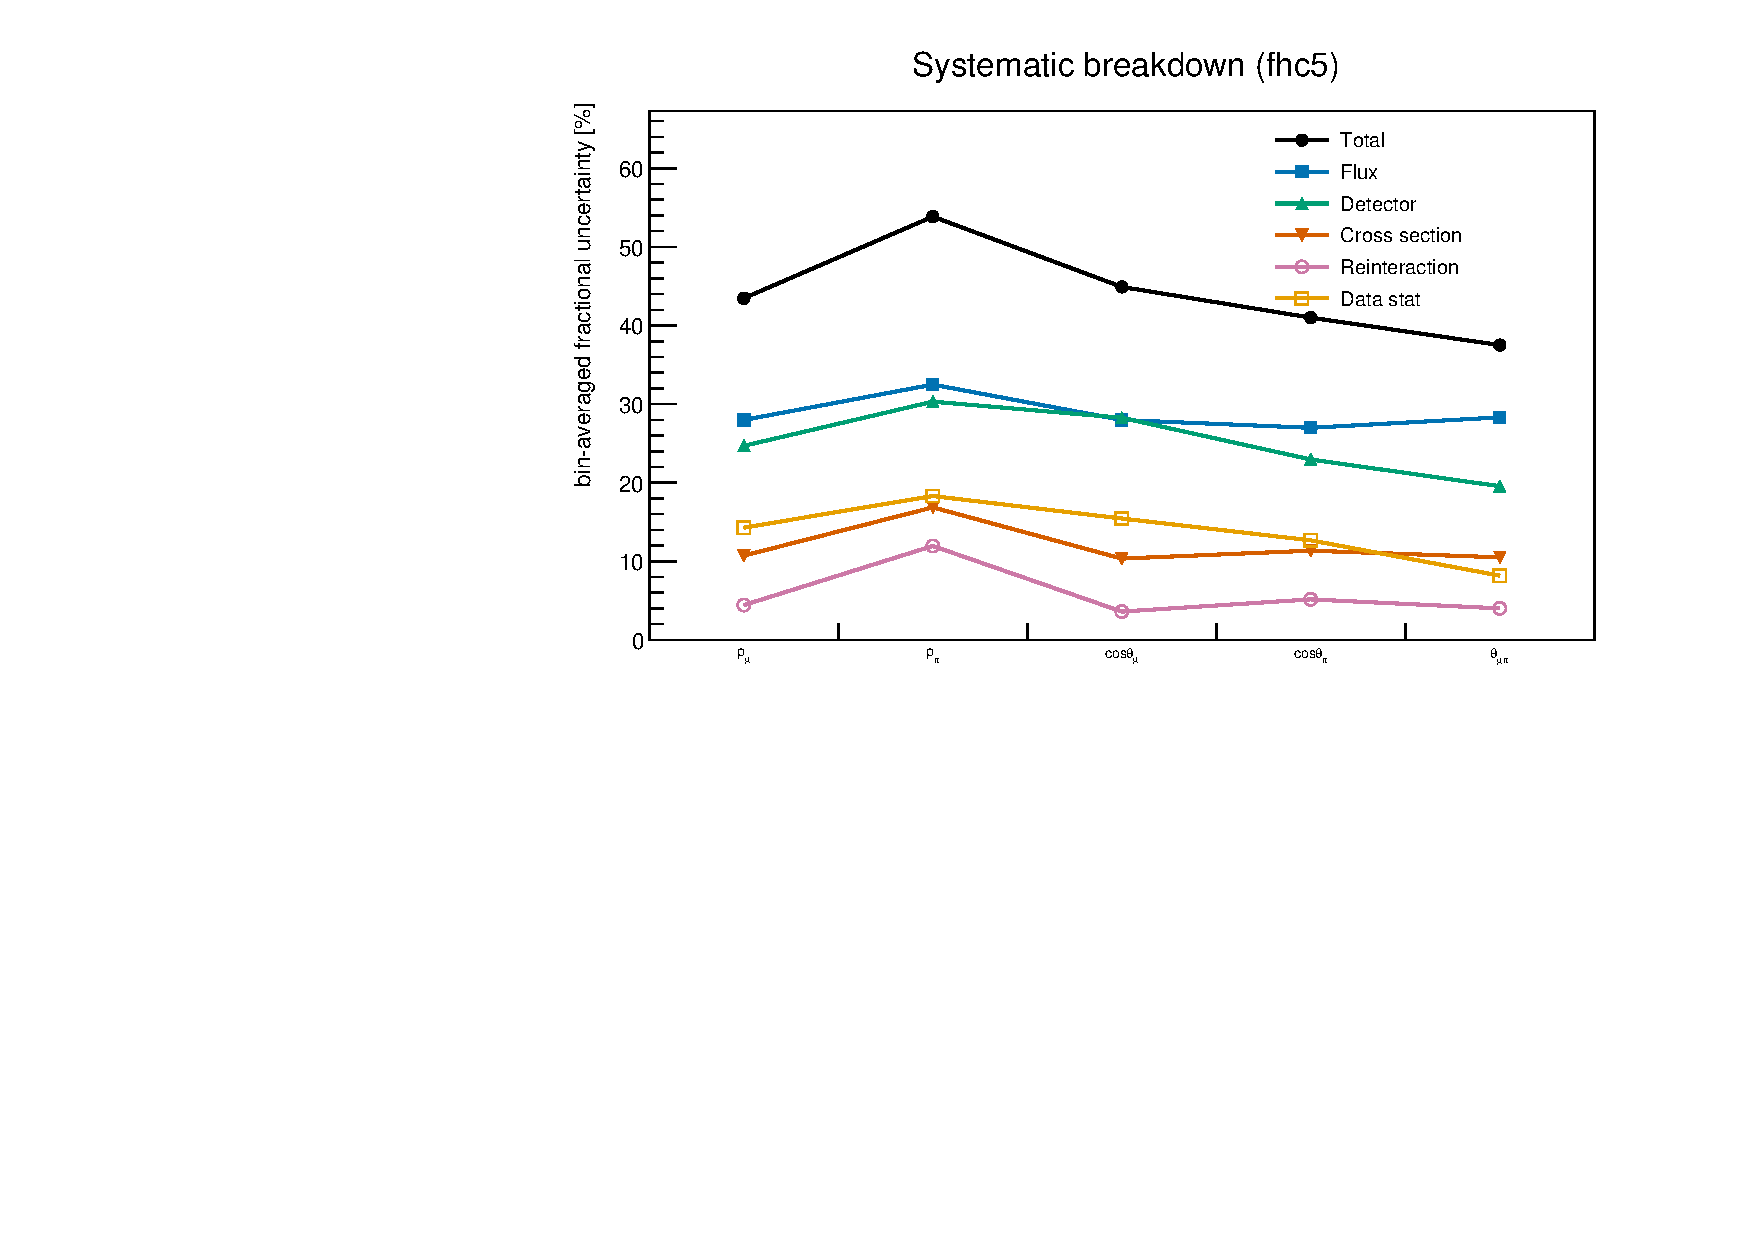
\includegraphics[width=\textwidth]{fw_systbreak_fhc}
  \column{.5\textwidth}\small
  Bin-averaged fractional uncertainty, inclusive (\%):
  \begin{tabular}{lcc}
  \toprule
  Source & range & \\
  \midrule
  Flux (PPFX) & 24--34 & dominant \\
  Detector & 17--43 & $\sim$ flux for several obs. \\
  Cross section & 9--18 & \\
  Re-interaction & 3--12 & \\
  Data statistics & 7--20 & \\
  \midrule
  Total & 34--62 & \\
  \bottomrule
  \end{tabular}\\[4pt]
  \begin{itemize}\itemsep2pt
    \item the $\sim17\%$ reco-level flux is amplified by the unfolding operator; the lever is response conditioning, not the flux model
    \item all 51 extractions carry a full covariance including detector variations; $A_C$ and covariances released as text
  \end{itemize}
  \end{columns}
\end{frame}

% ---------------------------------------------------------------------------
\begin{frame}{Validation, and what the review found}
  \footnotesize
  \begin{columns}[T]
  \column{.5\textwidth}
  \textbf{Validation}
  \begin{itemize}\itemsep2pt
    \item fake-data closure: unfolded/realised truth $=1.016$ on average over the 18 inclusive extractions; all $p>0.8$
    \item 32-throw ensemble: pull widths $1.04$ ($p_\mu$), $0.96$ ($\cos\theta_\mu$), 68/95\% coverage recovered; $2.5\%$ negative bias stated, not corrected
    \item clean-cache rebuild of all 51 extractions is bit-identical
    \item five automated guards: normalisation manifest, systematics/file coupling, staleness, table consistency, blinding guard
  \end{itemize}
  \column{.5\textwidth}
  \textbf{Corrected since August} (all in the change log)
  \begin{itemize}\itemsep2pt
    \item beam-off scaled by an \emph{event} count instead of gates: EXT was $9.7\times$ too large ($128\to30$ FHC events); now per run period
    \item fake-data truth carried the CV weight twice ($1.6\%$ on closure)
    \item PPFX CV weight missing from count-level tables ($3$--$6\%$)
    \item one safe-weight rule everywhere; fake data re-thrown with it ($1\%$)
    \item $A_C$ applied twice to models; TKI computed about detector $z$ (both withdrawn and redone)
  \end{itemize}
  \alert{None of these touched the real-data path; several would have biased a real-data result.}
  \end{columns}
\end{frame}

% ---------------------------------------------------------------------------
\begin{frame}{Proton-tagged subsample}
  \begin{columns}[T]
  \column{.6\textwidth}
  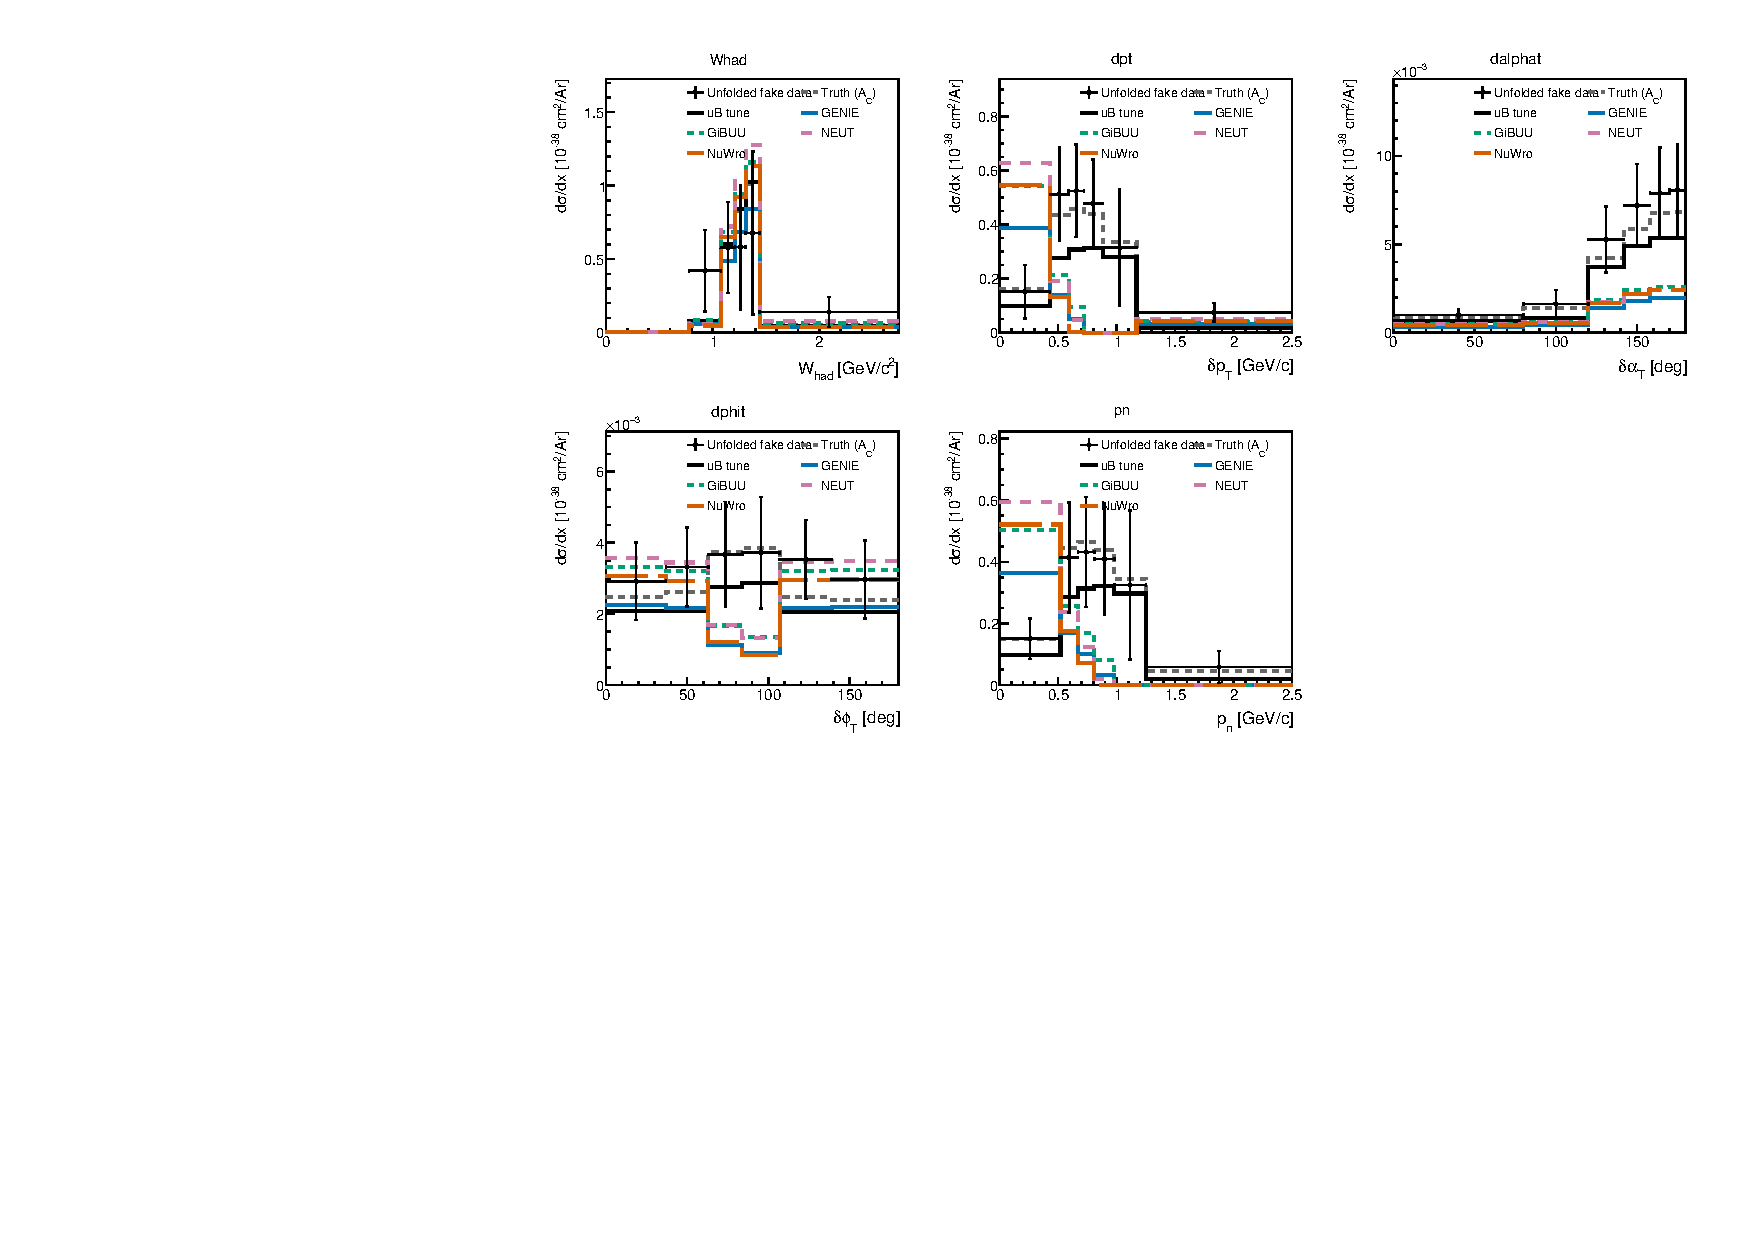
\includegraphics[width=\textwidth]{dsigma_ccpi1p_noW_FHC5}
  \column{.4\textwidth}\small
  \begin{itemize}\itemsep3pt
    \item inclusive selection $+$ a contained proton $>0.3$\GeVc; efficiency $11.4\%$, purity $\sim50\%$; strong cosmic rejector
    \item TKI ($\delta p_T$, $\delta\alpha_T$, $\delta\phi_T$, $p_n$) in two bins, beam frame; $W_{\rm had}$ in six
    \item single-nucleon STV prescription applied to the $\pi p$ system: $p_n$ is a proxy (stated limitation)
    \item generators: normalisation spread only; no FSI discrimination at this exposure
    \item headline: integrated total $0.63\pm0.31$ (FHC)
  \end{itemize}
  \end{columns}
\end{frame}

% ---------------------------------------------------------------------------
\begin{frame}{Control regions}
  \begin{columns}[T]
  \column{.55\textwidth}\scriptsize
  \begin{tabular}{@{}p{0.95cm}p{1.55cm}p{4.3cm}@{}}
  \toprule
  Region & Inversion & Role; $T=N^{\rm SR}/N^{\rm CR}$ of the target class \\
  \midrule
  CC$0\pi$ & $n_\pi=0$ & tests $0\pi$ feed-in; $T=0.03$, $\delta T/T=31\%$ (detector-limited) \\
  multi-$\pi$ & $n_\pi\ge2$ & diagnostic only; $T=2.5$ \\
  $\pi^0$ & shower veto fails & $\pi^0$ leakage; $T=0.02$, $\delta T/T=15\%$: strongest handle \\
  cosmic & $\theta_{\mu\pi}>2.6$~rad & beam-off norm.\ and shape; $41\%$ EXT purity, no fitted correction \\
  \bottomrule
  \end{tabular}\\[3pt]
  \begin{itemize}\itemsep1pt
    \item disjoint from the signal region event by event; multi-$\pi$ and $\pi^0$ overlap ($\sim\!40\%$ of multi-$\pi$)
    \item pseudo-data/prediction $0.99$--$1.10$ everywhere; full-stack test (MC$+$EXT$+$dirt) at unity
    \item per-region systematics incl.\ detector variations; transfer factors as correlated ratios (flux cancels to $2$--$3\%$)
  \end{itemize}
  \column{.45\textwidth}
  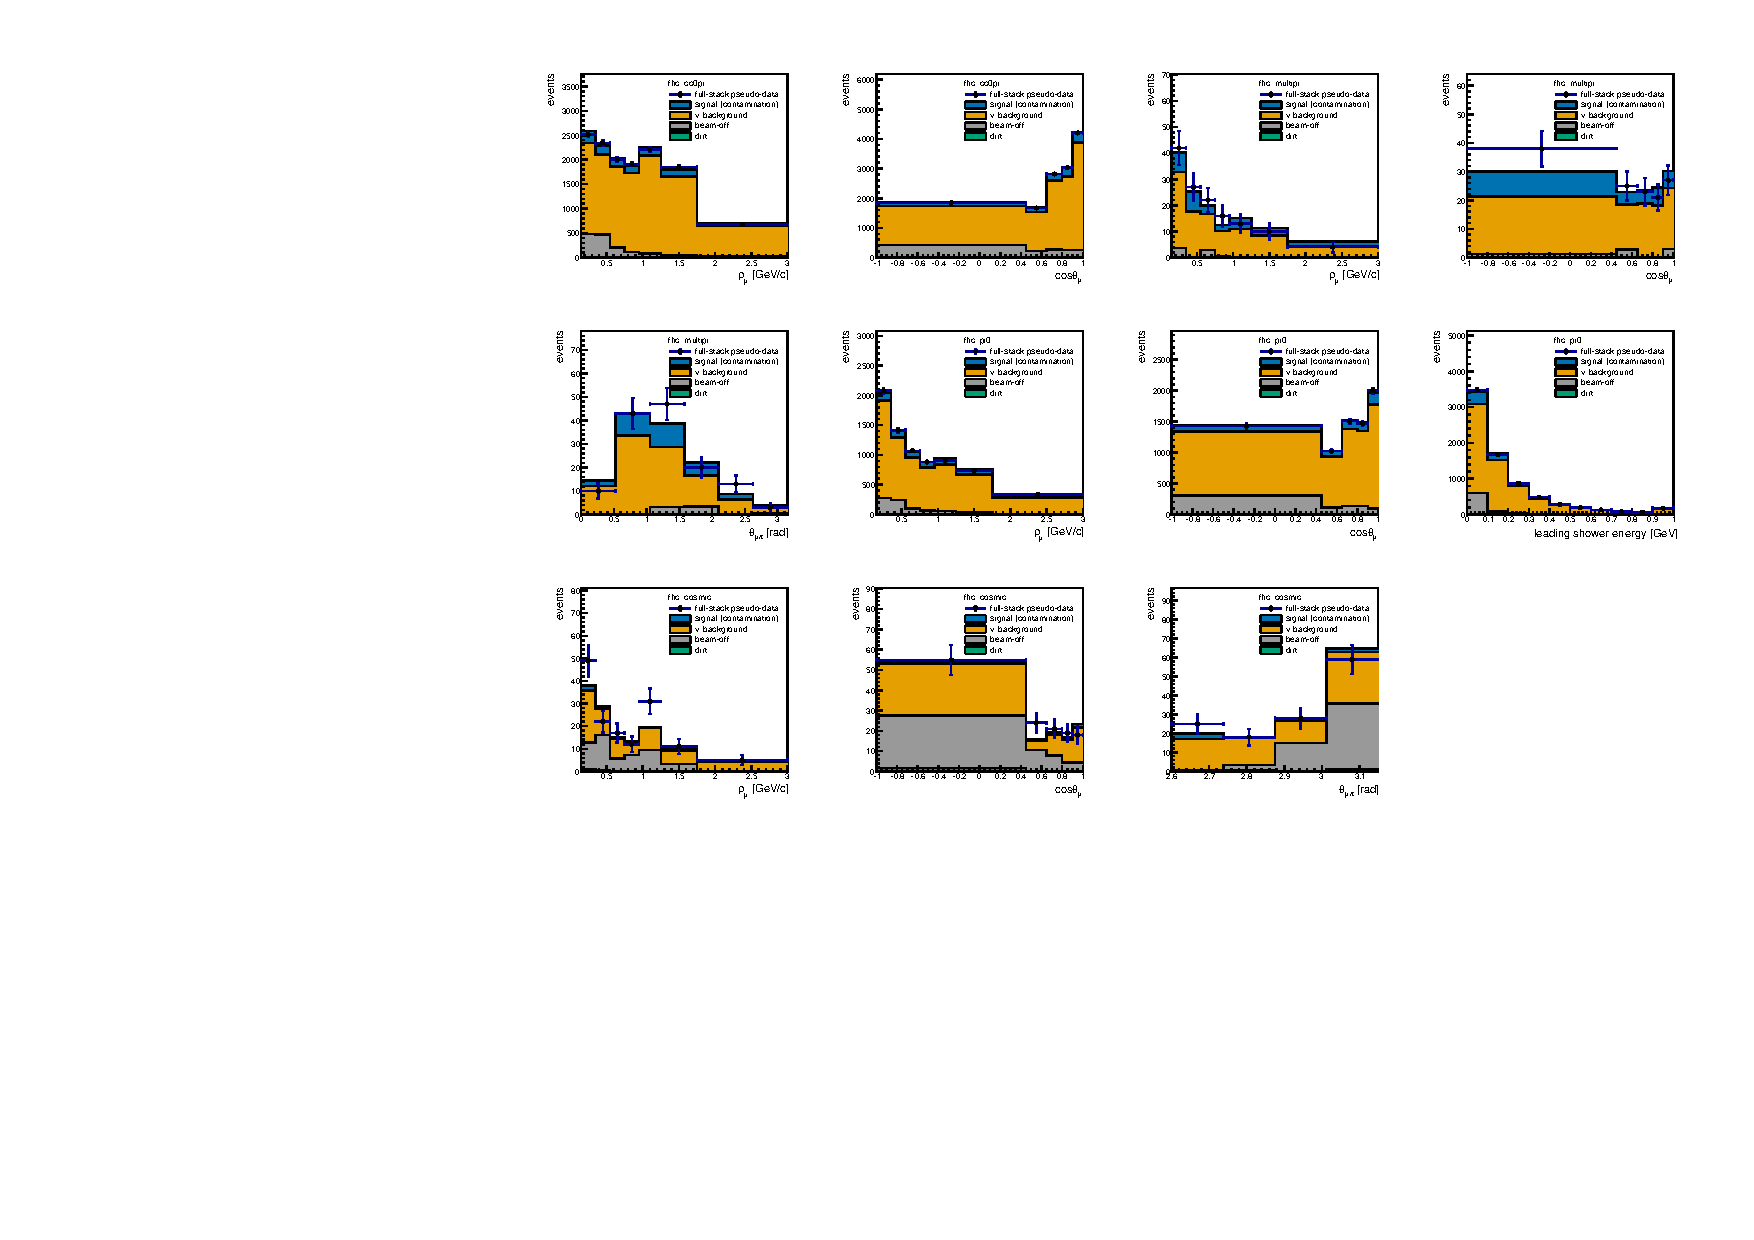
\includegraphics[width=\textwidth]{sideband_plots_fhc}\\
  {\scriptsize Frozen distributions and binning, FHC, full-stack pseudo-data in place of beam-on points.}
  \end{columns}
\end{frame}

% ---------------------------------------------------------------------------
\begin{frame}{Request to the collaboration}
  \begin{block}{Open the four inclusive control regions; the signal region and the proton-tagged regions stay blind}
  \small
  Frozen before opening: selections at branch level, run-dependent normalisation, beam-off scaling, displayed observables and binning, covariance, goodness-of-fit and the permitted responses.
  \end{block}
  \footnotesize
  \begin{columns}[T]
  \column{.5\textwidth}
  \textbf{Procedure} (to be ratified)
  \begin{itemize}\itemsep1pt
    \item FHC and RHC separately, combined as cross-check; data vs.\ MC$+$EXT$+$dirt
    \item pass: normalisation within $2\sigma$ (pre-fit predictive uncertainty) and shape $p>0.05$
    \item allowed: no change; added uncertainty; one-parameter normalisation of the target class (purity $>50\%$, LR test, transfer uncertainty added); else model revision and renewed approval
    \item forbidden: any signal cut or binning change; generator choice after inspection; bin-by-bin reweighting
  \end{itemize}
  \column{.5\textwidth}
  \textbf{Prerequisites}
  \begin{itemize}\itemsep1pt
    \item[$\checkmark$] tables from one release, checked automatically
    \item[$\checkmark$] definitions, overlap $=0$, plots and binning frozen
    \item[$\checkmark$] EXT gates released per run; pairings asserted
    \item[$\checkmark$] real beam-on files refused without \texttt{XSEC\_UNBLIND=1}
    \item[$\checkmark$] full-stack closure; region systematics incl.\ detector; transfer uncertainties
    \item[$\square$] ratification of the procedure
  \end{itemize}
  Before the signal region: PPFX-corrected flux constants confirmed; discrepancy treatment; clean-cache reproduction.
  \end{columns}
\end{frame}

% ---------------------------------------------------------------------------
\begin{frame}{Summary}
  \small
  \begin{itemize}\itemsep4pt
    \item A blind, fully validated extraction of $\nu_\mu+\bar\nu_\mu$ CC$1\pi^\pm$ cross sections on argon in the NuMI beam: total and six differential distributions in FHC, RHC and combined, with full covariances and released $A_C$ matrices.
    \item Two physics limits set the scope: the pion range saturates (two-bin $p_\pi$; no $W_{\pi p}$ shape), and $A_C$ is not norm preserving (the total is cut-and-count).
    \item Fake-data totals $1.03/0.93/0.98\times10^{-38}$~cm$^2$/Ar with $\sim\!41\%$ uncertainty, flux- and detector-limited.
    \item A sequence of normalisation and weighting defects was found by review and fixed; automated guards now stop each of them from recurring.
    \item \alert{We ask to open the four inclusive control regions under the frozen procedure.}
  \end{itemize}
  \vspace{4pt}
  \footnotesize Documents: analysis note (Draft 1.3), technical supplement, change log; data release in \texttt{report/data\_release/}.
\end{frame}

\end{document}
